\section{Relation to an earlier draft}
\label{app:earlier}

An unpublished 2023 draft of this work reported results for an earlier implementation of the alignment loss. In that implementation the loss could not influence the generator: the predicted spectrogram was decoded from the argmax of the transformer's logits inside a function that ran without gradient tracking, so no gradient reached the transformer, and the only parameters the loss touched, those of its two feature extractors, were not in the optimizer. All numbers in that draft are superseded by this paper. The experiments reported here were rerun with a new implementation in which the gradient does reach the transformer (\cref{sec:pal-loss}); with that path in place, the loss the draft intended does not improve timing (\cref{sec:res-loss}).

\section{FlashDot example and metric check values}
\label{app:extra}

\begin{figure}[h]
  \centering
  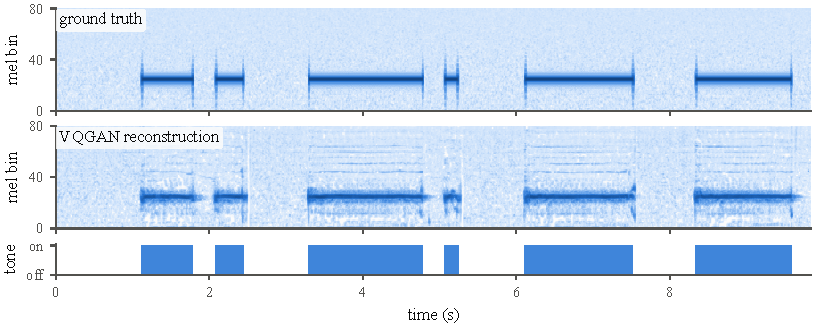
\includegraphics[width=0.85\linewidth]{figures/flashdot_example.pdf}
  \caption{A FlashDot clip: ground-truth spectrogram, its VQGAN reconstruction with the public VAS codebook, and the tone label. The reconstruction keeps the timing (tone F1 0.970 over the development split) and adds codebook texture, so it bounds what any code model with this decoder can reach.}
  \label{fig:flashdot}
\end{figure}

\begin{table}[h]
  \centering
  \caption{Response of candidate metrics to known delays, mean over 200 FlashDot development clips. Arrows give the direction of a better score.}
  \label{tab:sensitivity}
  \small
  \begin{tabular}{lccccc}
    \toprule
    Comparison & DTW $\downarrow$ & Mel L1 $\downarrow$ & Onset F1 $\uparrow$ & Env.\ corr.\ $\uparrow$ & $|$Lag$|$ (ms) $\downarrow$ \\
    \midrule
    Delay 0\,ms   & 0     & 0.000 & 1.00 & 1.00  & 0 \\
    Delay 23\,ms  & 69    & 0.032 & 1.00 & 0.75  & 23 \\
    Delay 46\,ms  & 138   & 0.035 & 1.00 & 0.32  & 46 \\
    Delay 93\,ms  & 271   & 0.036 & 1.00 & 0.01  & 93 \\
    Delay 186\,ms & 527   & 0.040 & 0.05 & 0.02  & 186 \\
    Delay 372\,ms & 1034  & 0.045 & 0.13 & $-0.01$ & 372 \\
    Delay 743\,ms & 1968  & 0.052 & 0.14 & $-0.04$ & 743 \\
    \midrule
    Other clip    & 10582 & 0.054 & 0.14 & 0.01  & 470 \\
    \bottomrule
  \end{tabular}
\end{table}

\clearpage
\section{Hyperparameters}
\label{app:hparams}

\begin{table}[h]
  \centering
  \caption{Hyperparameters. Values are those of the reported runs; red entries are not yet fixed.}
  \label{tab:hparams}
  \small
  \begin{tabular}{llc}
    \toprule
    Component & Setting & Value \\
    \midrule
    Training critic & encoder blocks / kernel / channels & 2 / 5 / 256 \\
           & embedding dimension, normalization & 128, L2 per frame \\
           & group norm groups, mel pooling & 8, $\times 4$ \\
    Held-out critic & blocks / kernel / channels, seed & 3 / 3 / 384, 1 \\
           & audio input (FlashDot / VAS) & mel / 8 bands \\
    \midrule
    Stage 1 & $K$, $\tau$, $\sigma$ & 10, 0.1, 0 \\
            & $S$ (FlashDot / VAS) & 4 / 8 \\
            & reduction & $-\frac{1}{S}\sum_s \log W_s$ \\
            & probability of ground-truth audio & 0.3 \\
            & optimizer & AdamW, lr $10^{-3}$, wd $10^{-4}$ \\
            & steps (FlashDot / VAS), batch & 2000 / 3000, 32 \\
            & selection & lowest dev loss \\
    \midrule
    PAL as a loss & $K$, $S$, $\tau$, $\sigma$ & 8, 4, 0.1, 1 \\
    (FlashDot) & reduction & $-\log \frac{1}{S}\sum_s W_s$ \\
            & decoding & straight-through \\
            & window columns $c$, margin $m$ & 12, 1 \\
            & examples with PAL per batch & 4 of 8 \\
            & PAL weight $\beta$ & 1 \\
            & $p_{\mathrm{keep}}$ (CE pass), $p^{\mathrm{PAL}}_{\mathrm{keep}}$ & $\{1, 0.5\}$, $\{1, 0.5, 0\}$ \\
            & optimizer & AdamW, lr $3 \times 10^{-4}$, $\beta = (0.9, 0.95)$, wd 0.01 \\
            & schedule, gradient clipping & 200 warm-up steps, cosine decay; 1.0 \\
            & steps, batch & 2000 (3000 teacher-forced PAL), 8 \\
    \midrule
    FlashDot GPT & layers / width / heads & 6 / 384 / 6 \\
    \midrule
    Self-training & rounds, steps per round & 2, 300 (FlashDot) / 150 (VAS) \\
            & clips per round, candidates $N$ & 400, 8 (FlashDot) / 256, 4 (VAS) \\
            & batch, ground-truth share & 8 (FlashDot) / 4 (VAS), 0.5 \\
            & trained parameters & all (FlashDot) / LoRA $r = 16$, $\alpha = 16$ (VAS) \\
            & initialization & CE, corrupted prefix (FlashDot) / public model (VAS) \\
            & optimizer & AdamW, lr $10^{-4}$, $\beta = (0.9, 0.95)$, wd 0.01 \\
            & candidate scoring & training critic, $\sigma = 1$ \\
    \midrule
    Sampling & top-$k$, temperature & 100, 1.0 \\
             & re-ranking samples $N$ (FlashDot / VAS) & 8 / 4 \\
    \midrule
    Seeds & FlashDot / VAS & 3 (test) / 1 \\
    \bottomrule
  \end{tabular}
\end{table}

\section{VAS sample}

\begin{figure}[h]
  \centering
  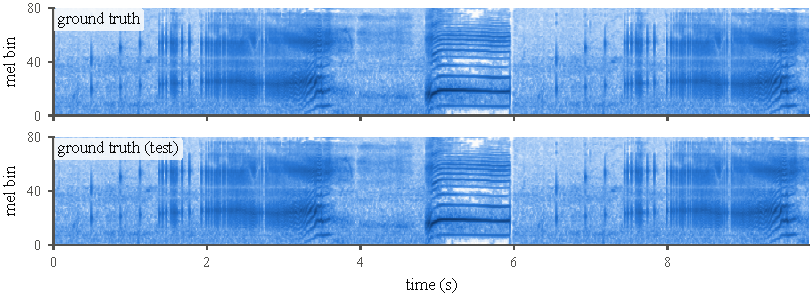
\includegraphics[width=\linewidth]{figures/vas_samples.pdf}
  \caption{One VAS test clip (the clip with the median $|$lag$|$ gain from best-of-4 re-ranking). Its $|$lag$|$ is 116\,ms for the single sample and 81\,ms for the best of four. VAS audio is dense, and timing differences of this size are hard to see in a spectrogram, which is why we report onset and envelope measures.}
  \label{fig:vas-samples}
\end{figure}
